% Part 1: Plot the first coordinate against the line number in the dataset.
% Part 1: Choose a delay Δn of rows and plot the coordinate against its delayed version.
% Part 1: How many coordinates are sufficient so that the periodic manifold is embedded correctly?

% Part 2: Describe the result in comparison to the attractor in x, y, z coordinates.
% Part 2: Do the time-delay embedding for the z coordinate. Why do you think this fails?

% Bonus: Discussed how and why you chose the values of L and ϵ?
% Bonus: Approximate the vector field on the Lorenz attractor embedding from part 2, using RBF.
% Bonus: Solve the system and compare the trajectories.

In Figure \ref{task4_1}, plotting the number of lines against data from the first column reveals a fluctuating curve. In Figure \ref{task4_2}, the data from the first column is graphed against itself with a 5-unit delay.


\begin{figure}[H]
\centering
    \begin{subfigure}{0.45\textwidth}
        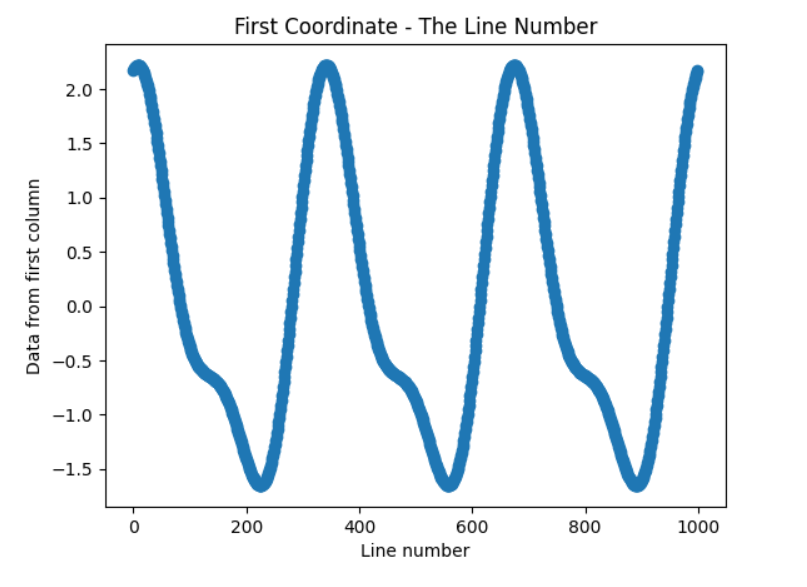
\includegraphics[width=\linewidth]
        {images/task4_wlinenumber.png}
        \caption{First Coordinate - The Line Number}
        \label{task4_1}
    \end{subfigure}
    \begin{subfigure}{0.45\textwidth}
        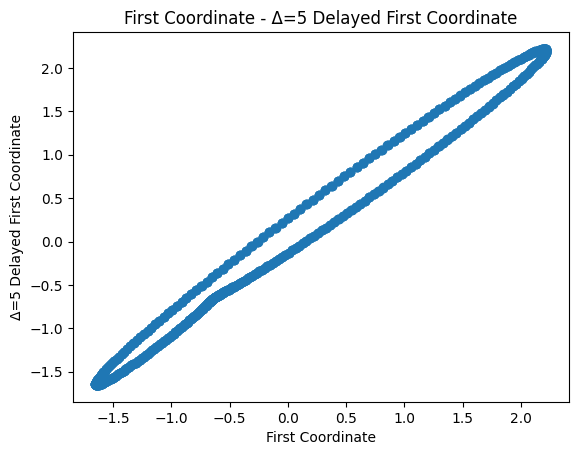
\includegraphics[width=\linewidth]
        {images/task4_d5delayedfirstcoordinate.png}
        \caption{First Coordinate - $\Delta$=5 Delayed First Coordinate}
        \label{task4_2}
    \end{subfigure}
    
    \caption{}
\end{figure}

According to the Time-delay embedding explanation in the exercise sheet, for a 1-dimensional manifold, we require \textbf{3 coordinates} (d=1 from $2d+1$) to ensure accurate embedding of the manifold. However, in Figure \ref{task4_2} with our current graph and $\Delta=5$, there is no collapse, indicating that it can be considered correctly embedded with just 2 coordinates. \\

In \textbf{part 2} of this exercise, we initiated the Lorenz Attractor as implemented in Exercise 4, with its graph displayed in Figure \ref{task4_3}. The values are stored in the variable \texttt{coordinates}. For Figure \ref{task4_4}, we utilized the x coordinate from this variable. Shifting x values by 5 units for the y-axis and 10 units for the z-axis resulted in a similarly shaped curve, affirming the correctness of Takens' theorem. However, when using z values from \texttt{coordinates}, the shape diverges from Figure \ref{task4_3}. Collapsation of two circles, originally distinct in \ref{task4_2}, indicates an embedding failure.


\begin{figure}[H]

    \begin{subfigure}{0.45\textwidth}
        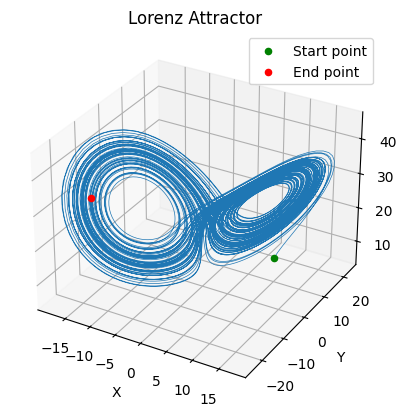
\includegraphics[width=\linewidth]{images/task4_lorenz.png}
        \caption{Lorenz Attractor which was in the Exercise 4}
        \label{task4_3}
    \end{subfigure}
    \centering

    \begin{subfigure}{0.45\textwidth}
        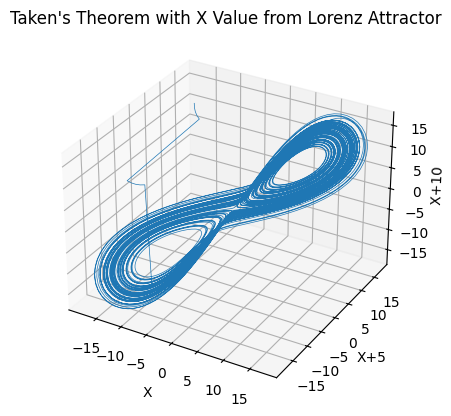
\includegraphics[width=\linewidth]{images/task4_takensX.png}
        \caption{Using only X values from Lorenz Attractor}
        \label{task4_4}
    \end{subfigure}
    \begin{subfigure}{0.45\textwidth}
        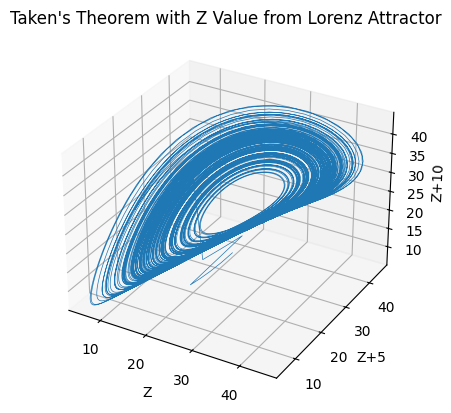
\includegraphics[width=\linewidth]
        {images/task4_takensZ.png}
        \caption{Using only Z values from Lorenz Attractor}
        \label{task4_5}
    \end{subfigure}

    \caption{}
\end{figure}






